\documentclass[
	aspectratio=169, % Uncomment to use an aspect ratio of 16:9 (160 mm by 90 mm)
	%aspectratio=43, % Uncomment to use an aspect ratio of 4:3 (128mm by 96mm)
	t, % Top align all slide content by default
	onlytextwidth, % Typeset content in columns at text width
	10pt, % Default font size, use 10pt for the 16:9 aspect ratio and 8pt for the 4:3 aspect ratio
]{beamer}
\usetheme{Imperial}
\usepackage{url}

\author[Colin Cotter]{Prof. Colin Cotter}
\institute{Department of Mathematics, Imperial College London}
\DeclareMathOperator{\diff}{d\!}
\DeclareMathOperator{\Div}{div}
\DeclareMathOperator{\Id}{Id}
\DeclareMathOperator{\Ro}{Ro}
\DeclareMathOperator{\ccurl}{curl}
\DeclareMathOperator{\ddiv}{div}
\DeclareMathOperator{\Tr}{Tr}
\newcommand{\pp}[2]{\frac{\partial #1}{\partial #2}} 
\newcommand{\Hcurl}{H(\operatorname{curl})}
\newcommand{\Hdiv}{H(\operatorname{div})}
\newcommand{\comment}[1]{}
\newcommand{\jump}[1]{\left[\!\left[ #1 \right]\!\right]}
\title[AMMP]{Applied Mathematics and Mathematics Physics section}

\begin{document}

\date{9th October 2024}

% Blue background title slide example

\begingroup
	\setbeamercolor{background canvas}{bg=ICLBlue} % Slide background color
	\setbeamercolor{title page title}{fg=white} % Title text color
	\setbeamercolor{title page subtitle}{fg=white} % Subtitle text color
	\setbeamercolor{author}{fg=white} % Author(s) text color
	\setbeamercolor{date}{fg=white} % Date text color
	\setbeamertemplate{title page}[logo]{ICL_Logo_White.pdf} % Imperial logo color, use 'ICL_Logo_White.pdf' for white and 'ICL_Logo_Blue.pdf' for blue
	\frame[plain, s]{\titlepage} % Output the title page with no footer ('plain') and vertically distributed text ('s')
\endgroup

\frame{
  \frametitle{Research focus in AMMP}
      \begin{columns}[T] % [T] ensures correct vertical alignment
        \begin{column}{0.48\linewidth} % Left column\
  \vfill
  \begin{itemize}
  \item Fluid Dynamics
  \item Applied Analysis and Numerical Analysis
  \item Dynamical Systems
  \item Biomathematics
  \item Mathematical Physics
  \end{itemize}
            \centerline{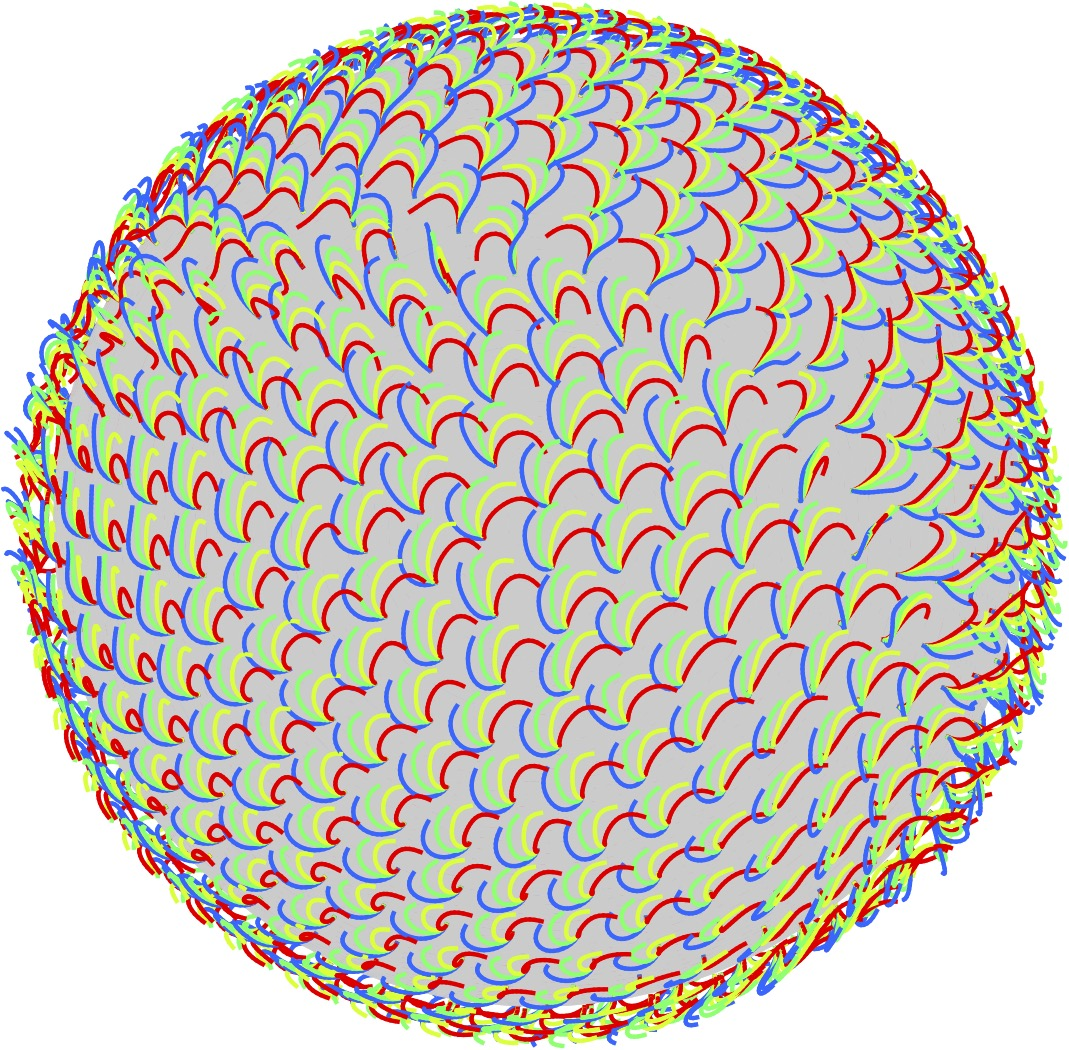
\includegraphics[width=3cm]{ActiveFilSphere}}
            \centerline{Spherical organism with active filamentsKeaveny}
            \centerline{(Eric Keaveny)}
  \vfill
        \end{column}
        \begin{column}{0.48\linewidth} % Left column
          \vspace{6mm}
          \centerline{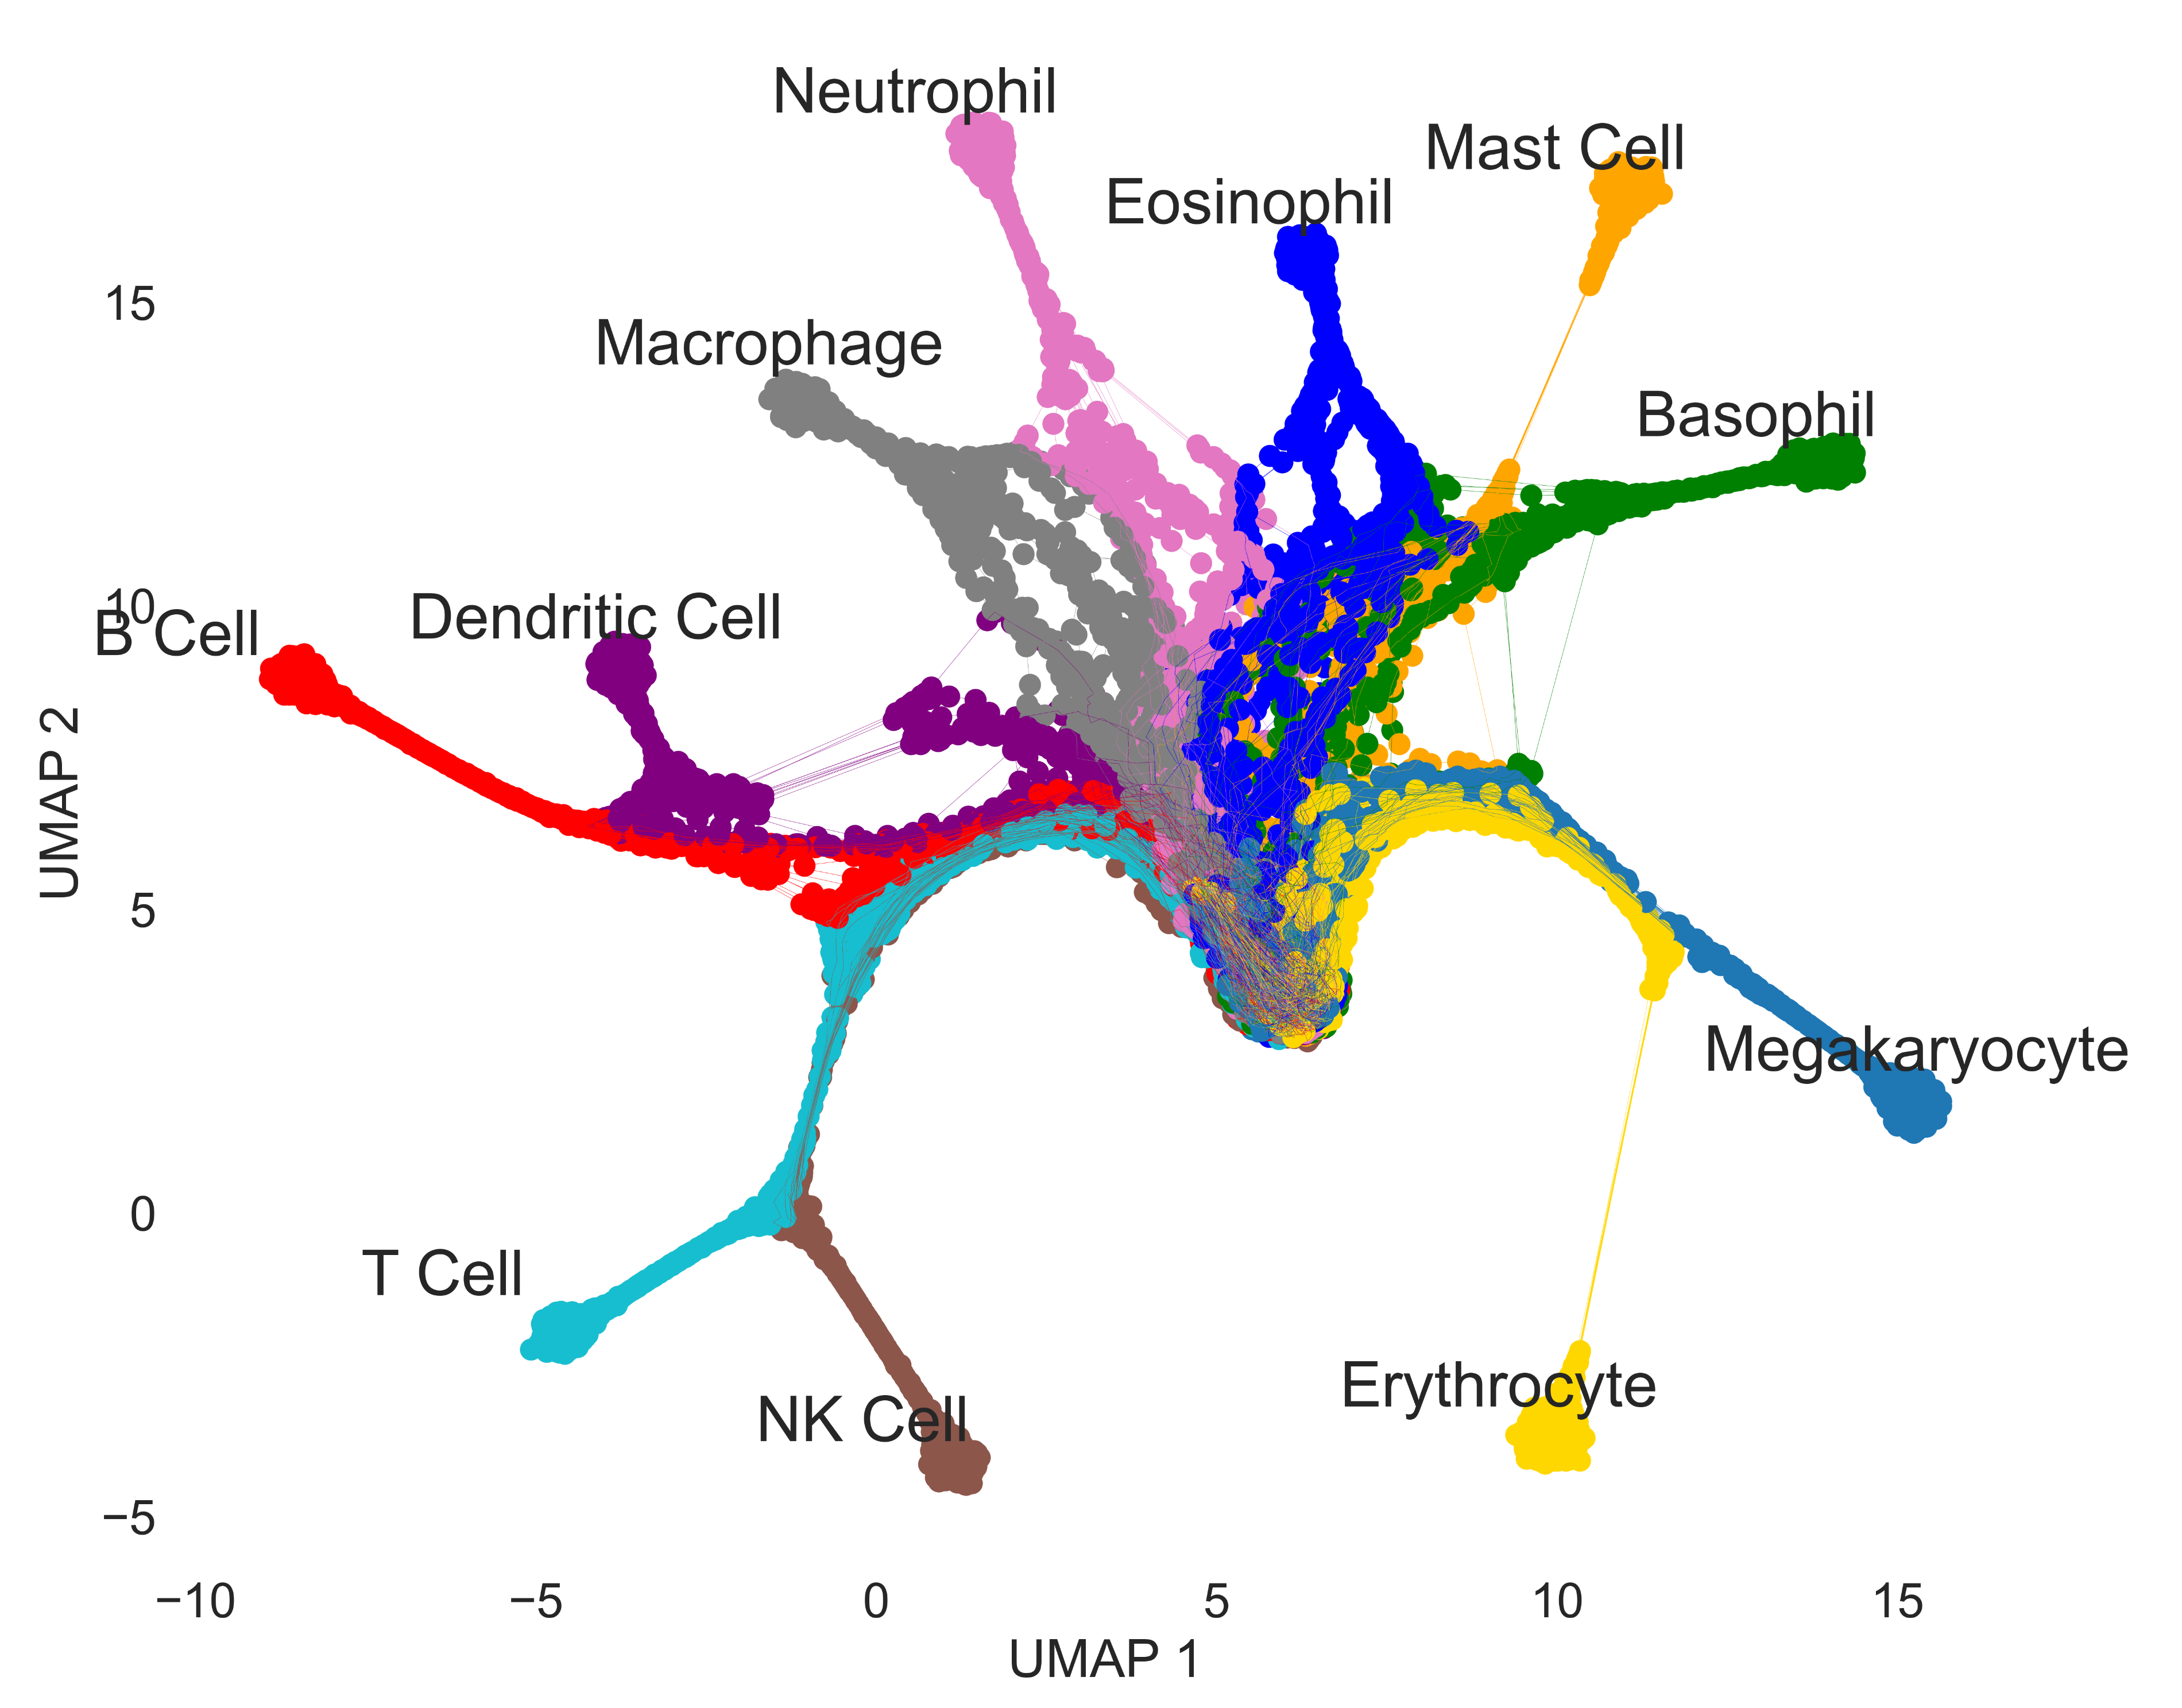
\includegraphics[width=6cm]{omer}}
          \centerline{3D visualisation of gene regulation (Omer Karin)}
        \end{column}
      \end{columns}
}

\frame{
  \frametitle{Fellowships}
    \begin{columns}[T] % [T] ensures correct vertical alignment
      \begin{column}{0.48\linewidth} % Left column
          \vfill
      \begin{itemize}
  \item Michele Coti Zelati - 2019-2027 Royal Society URF
  \item Eva-Maria Graefe - 2015-2024 Royal Society URF
  \item Philipp Thomas - 2020-2027 UKRI Future Leadership Fellow
  \item Greg Pavliotis - 2024-2025 Leverhulme Trust SRF
      \end{itemize}
      \vfill
    \end{column}
      \begin{column}{0.48\linewidth} % Left column
        \centerline{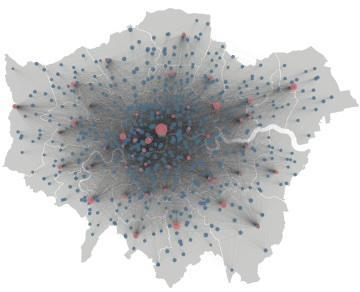
\includegraphics[width=6cm]{greg}}
        \centerline{Economic cost networks inferred from time series}
        \centerline{(Greg Pavliotis)}
      \end{column}
    \end{columns}
}

\frame{
  \frametitle{Meta4D (EPSRC programme grant)}
  Led by Richard Craster - metamaterials for cloaking that vary in time instead
  of space (Maths+Physics)
  \centerline{
    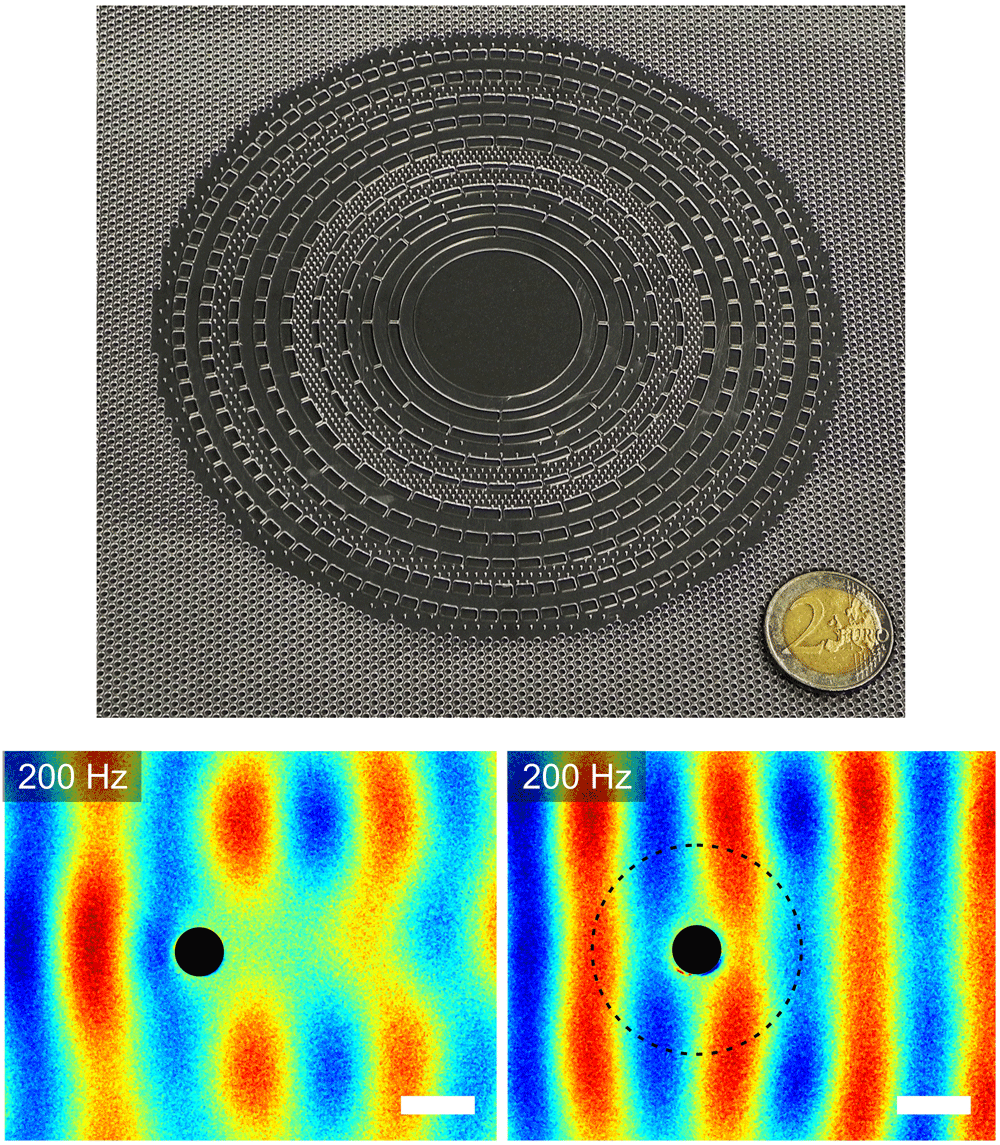
\includegraphics[width=6cm]{cloak}
  }
}

\frame{
  \frametitle{EPSRC investment in our Dynamical Systems group}
  \begin{itemize}
  \item Attractors in random dynamical systems with bounded noise: persistence, resilience and bifurcations (2024-2027)
  \item EPSRC Centre for Doctoral Training in Mathematics of Random
    Systems: Analysis, Modelling and Simulation (2019-2027)
  \item Mathematical Foundations of Intelligence: An "Erlangen
    Programme" for AI - (2024-2029)
  \end{itemize}
    \centerline{
      \includegraphics[width=4cm]{random}
    }
}

\frame{
  \frametitle{Proposal: Global Centre in Carbon Capture}
  Partners: Imperial, MIT, Tufts, UT Austin, UNIST S. Korea\\
  (Global Centres in clean energy and climate change)\\
  Previous bid: 2023\\
  \centerline{
    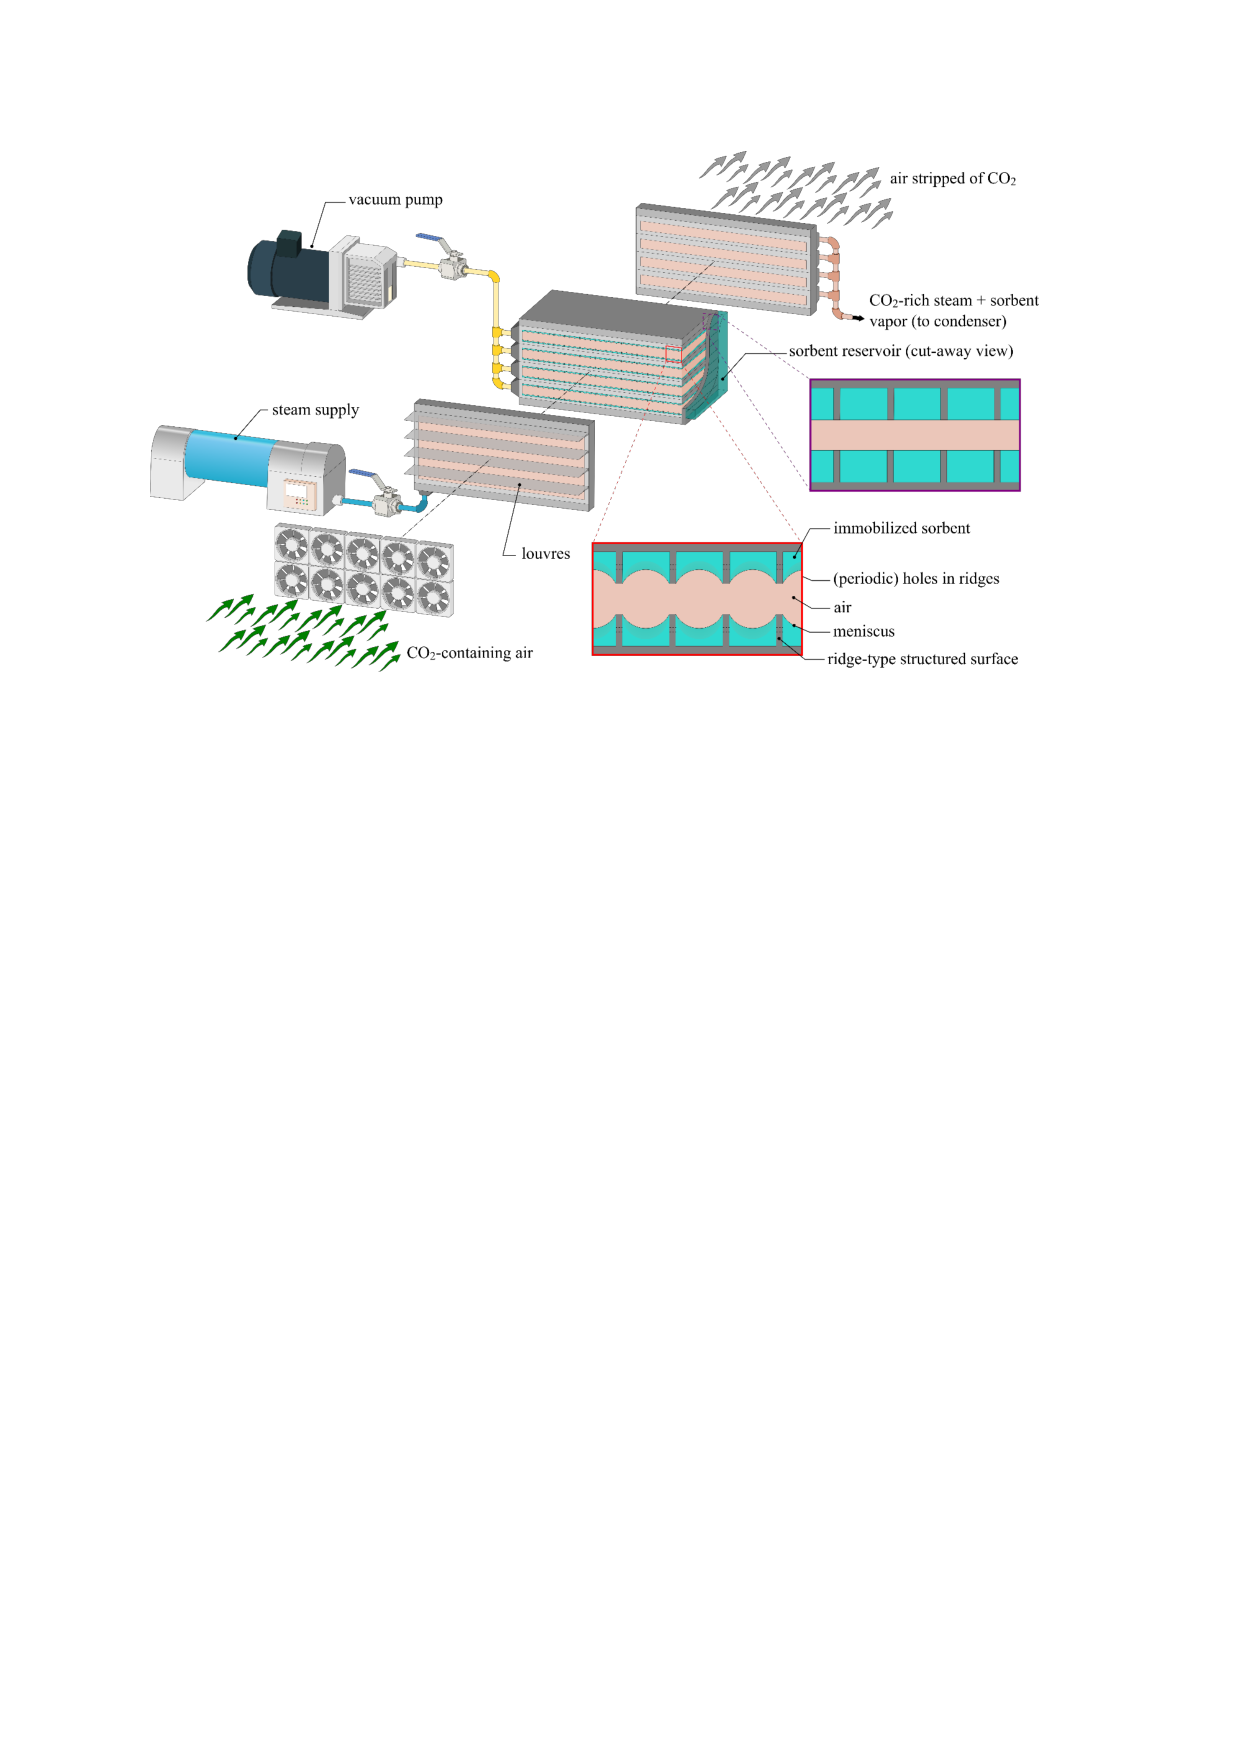
\includegraphics[width=10cm]{carbon.pdf}
  }
}

\frame{
  \frametitle{Other large programmes}
  \vfill
  \begin{columns}[T] % [T] ensures correct vertical alignment
    \begin{column}{0.48\linewidth} % Left column
      ERC Synergies grant: \\
      Stochastic Transport in Upper Ocean Dynamics\\
      (Dan Crisan and Darryl Holm)
      \centerline{
        \includegraphics[height=4cm]{stuod}
      }
    \end{column}
    \begin{column}{0.48\linewidth} % Left column
      EPSRC Physics of Life: Statistical Physics of Cognition \\
            (Mauricio Barahona Maths Co-I)
      \centerline{
        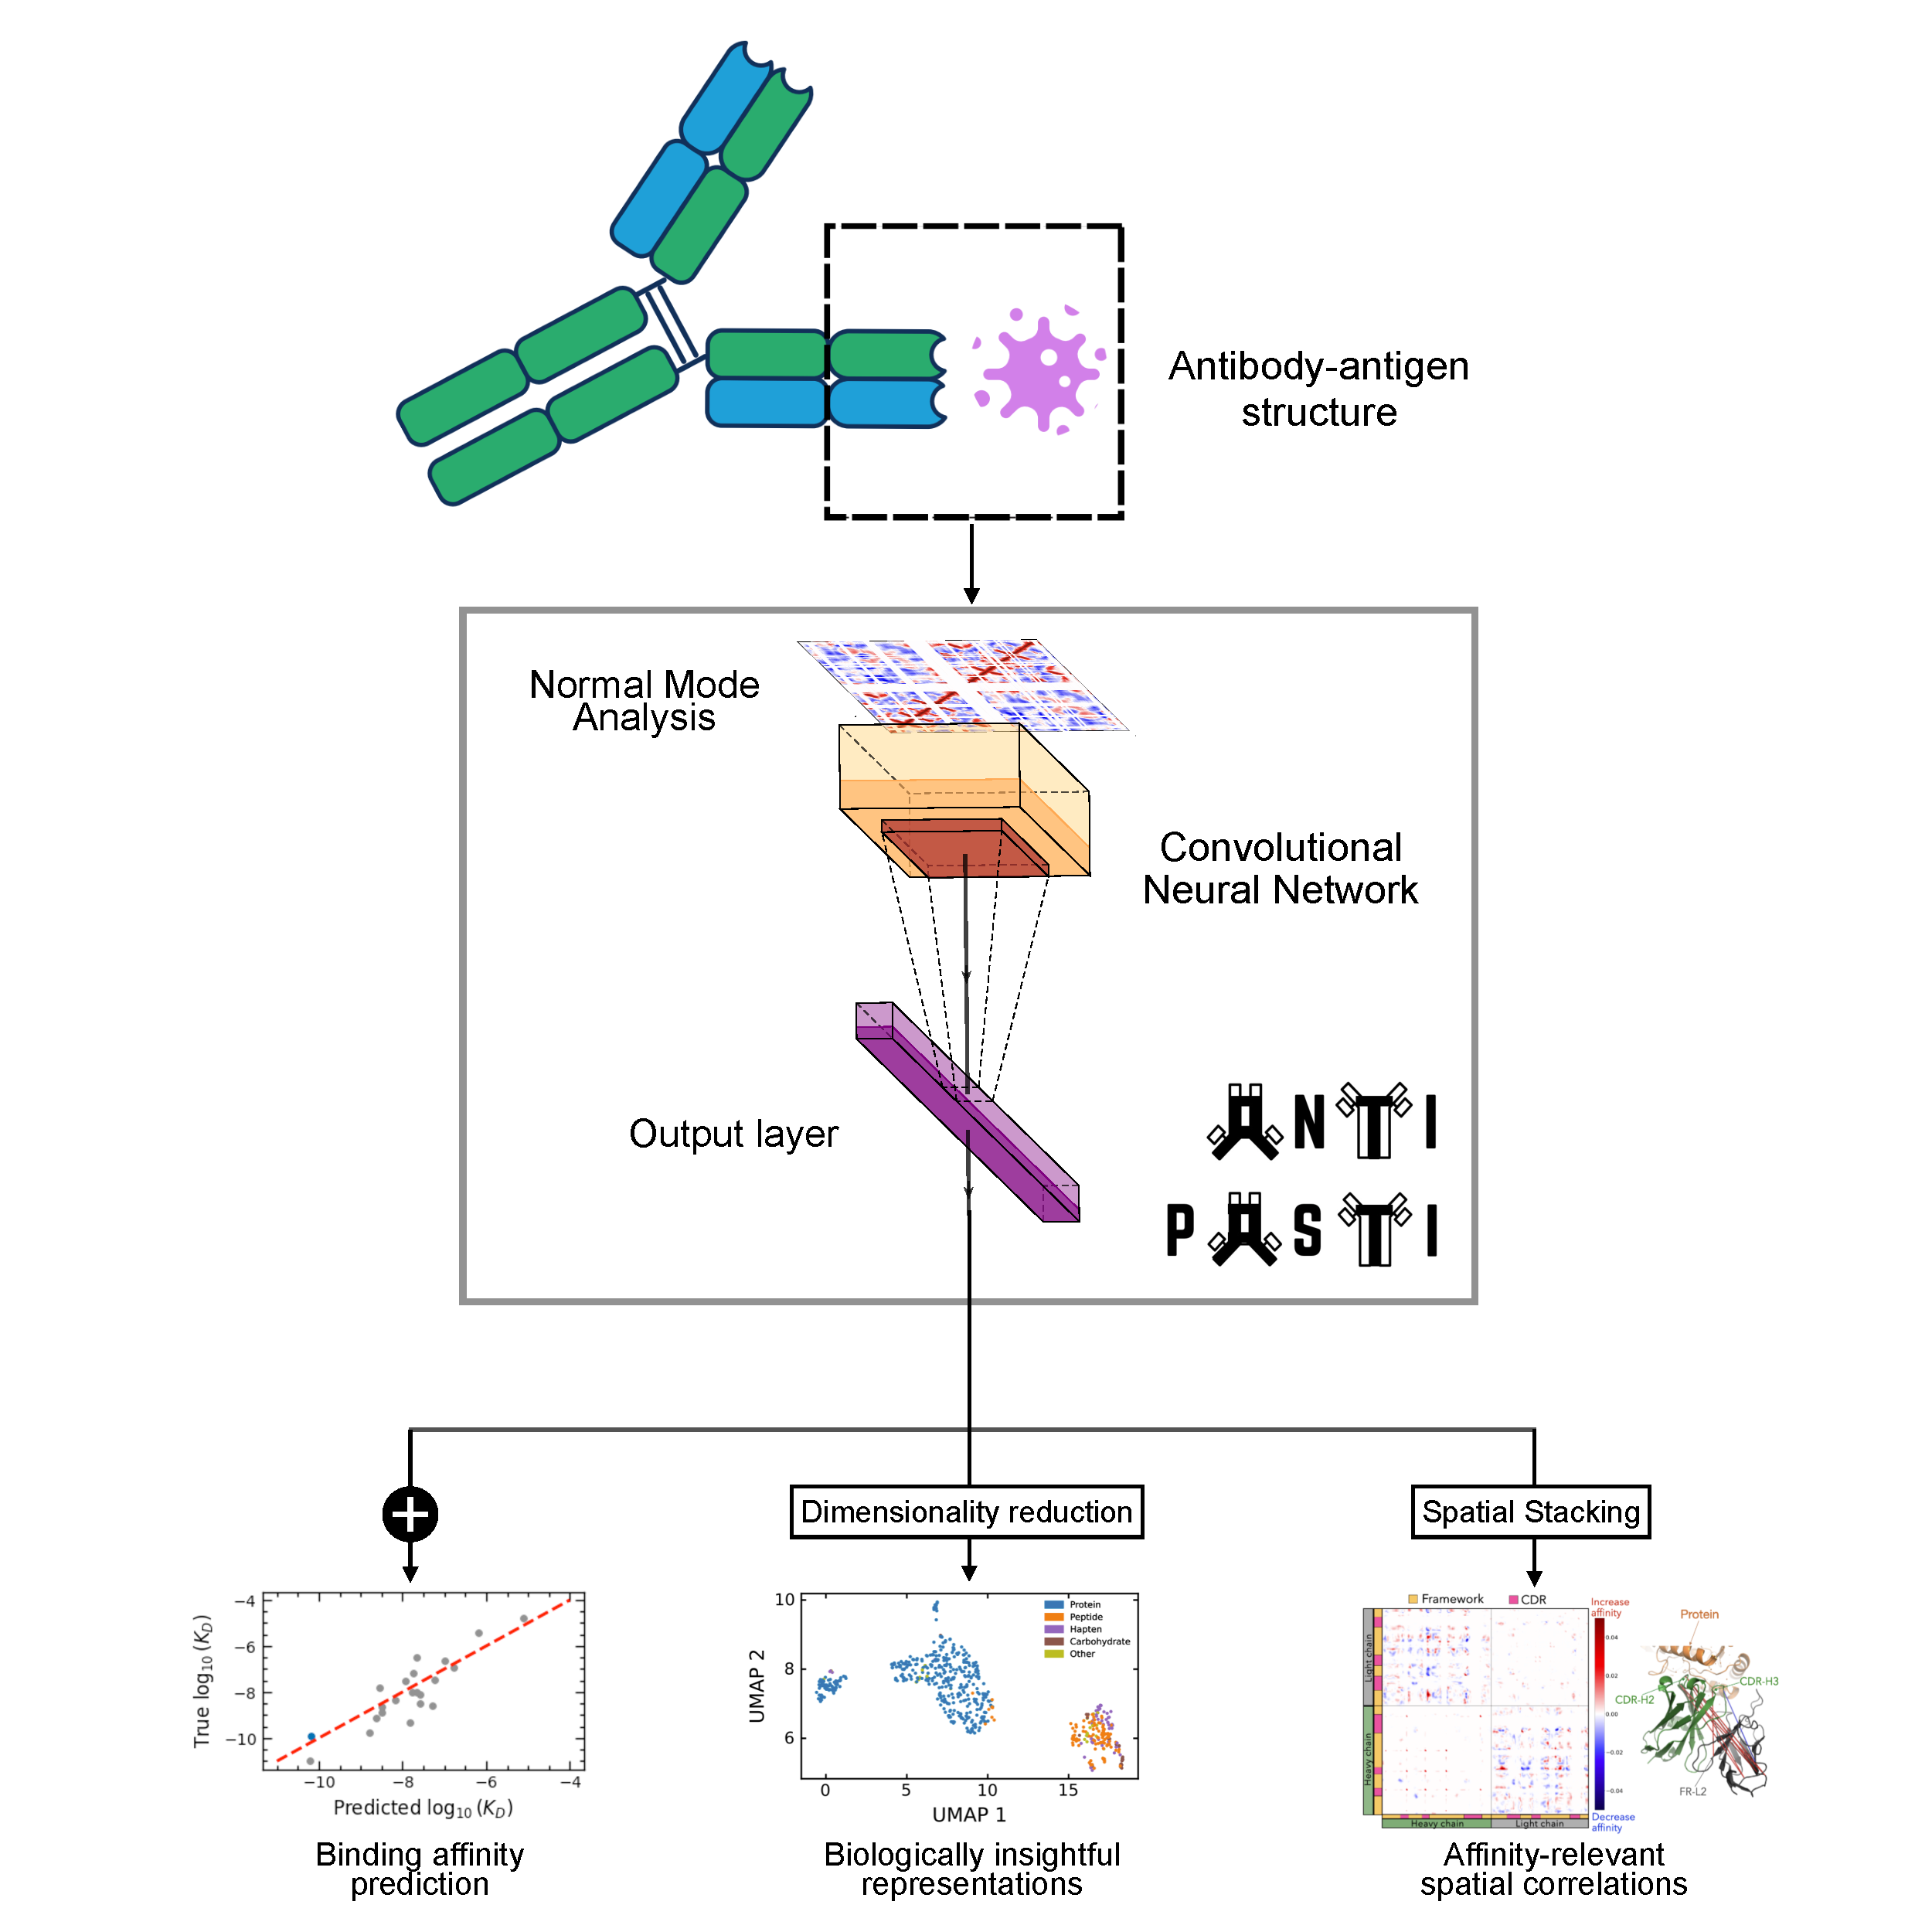
\includegraphics[height=4cm]{neurons}
      }
    \end{column}
  \end{columns}
    \vfill
}

\frame{
  \frametitle{Computational Science}
  ExCALIBUR
  \begin{itemize}
  \item (EPSRC) SysGenX - (David Ham, 2020-2021, 2022, 2025)
  \item (Met Office) APinTA PDEs - (Colin Cotter, 2021-2024)
  \end{itemize}
  Software for the future
  \begin{itemize}
    \item Firedrake: high performance, high productivity simulation
      for the continuum mechanics community (David Ham, 2022-2025)
  \end{itemize}
  \centerline{
    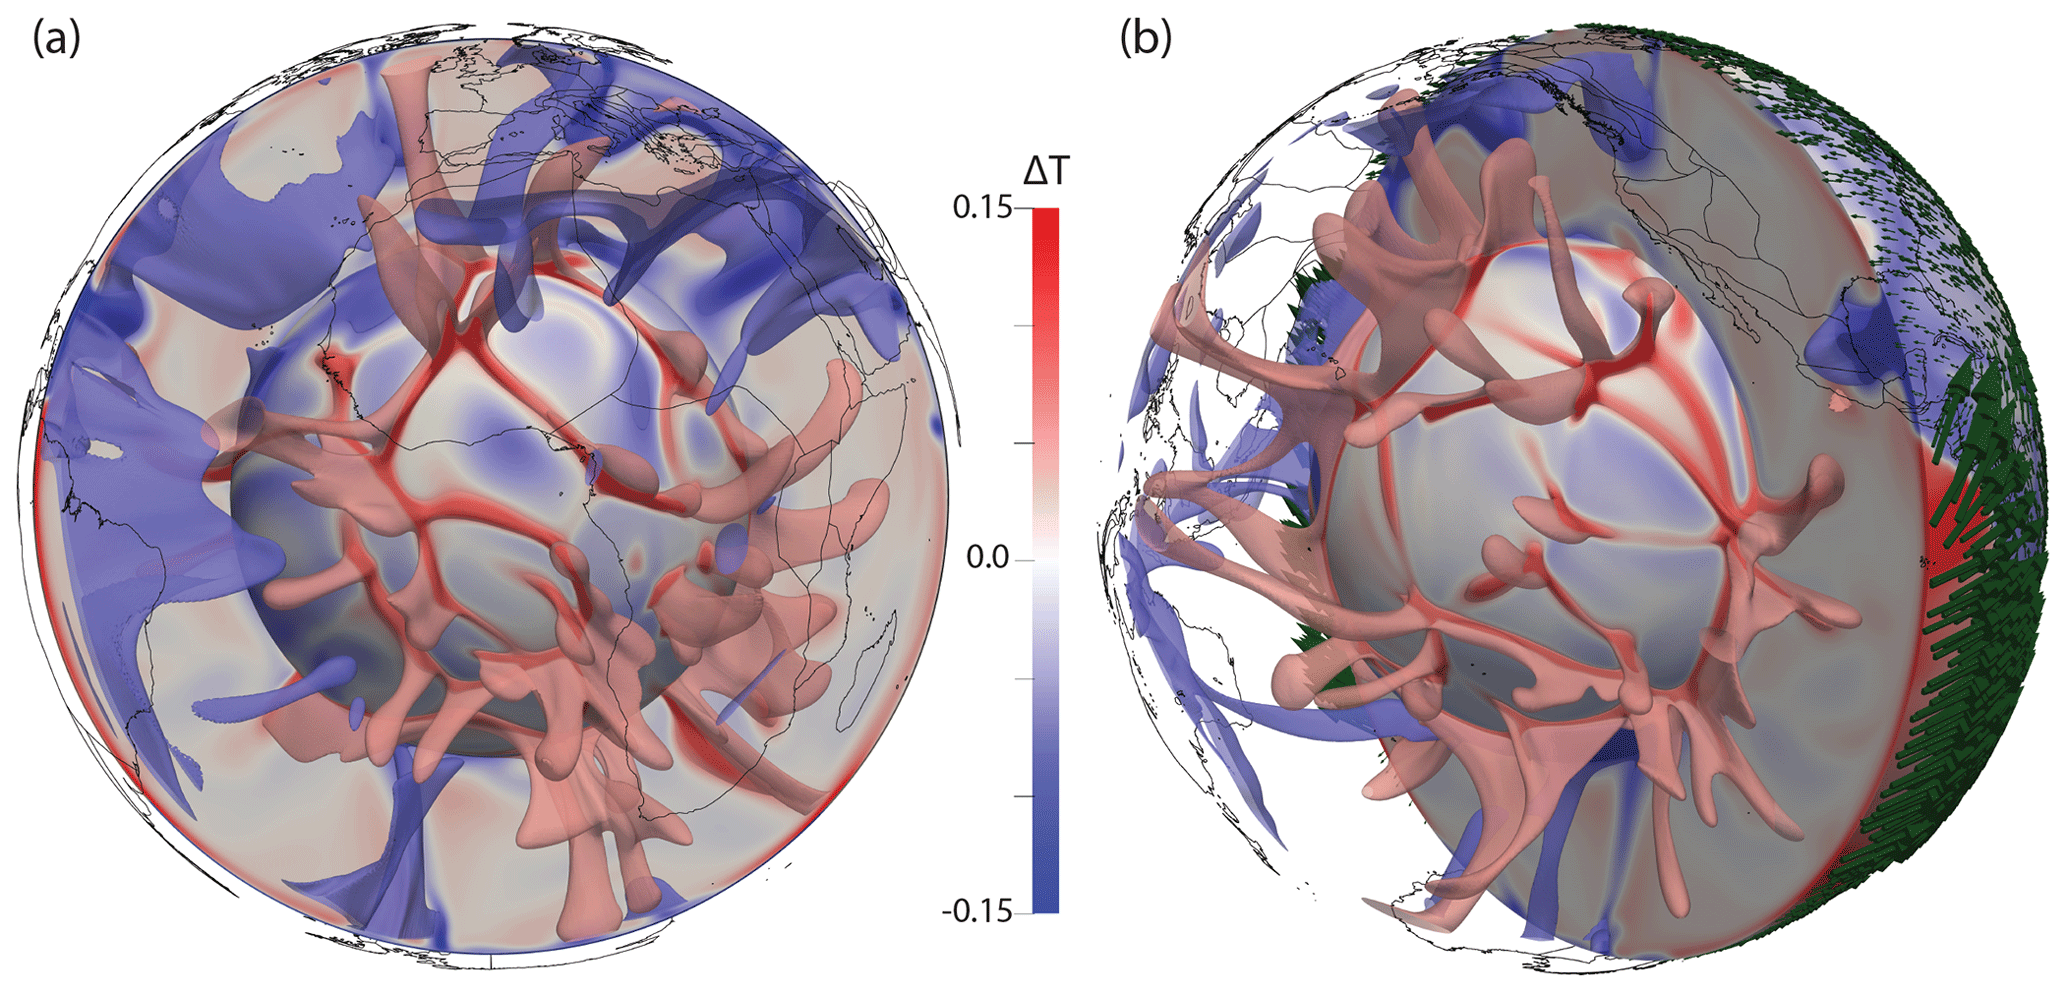
\includegraphics[height=3cm]{firedrake}
    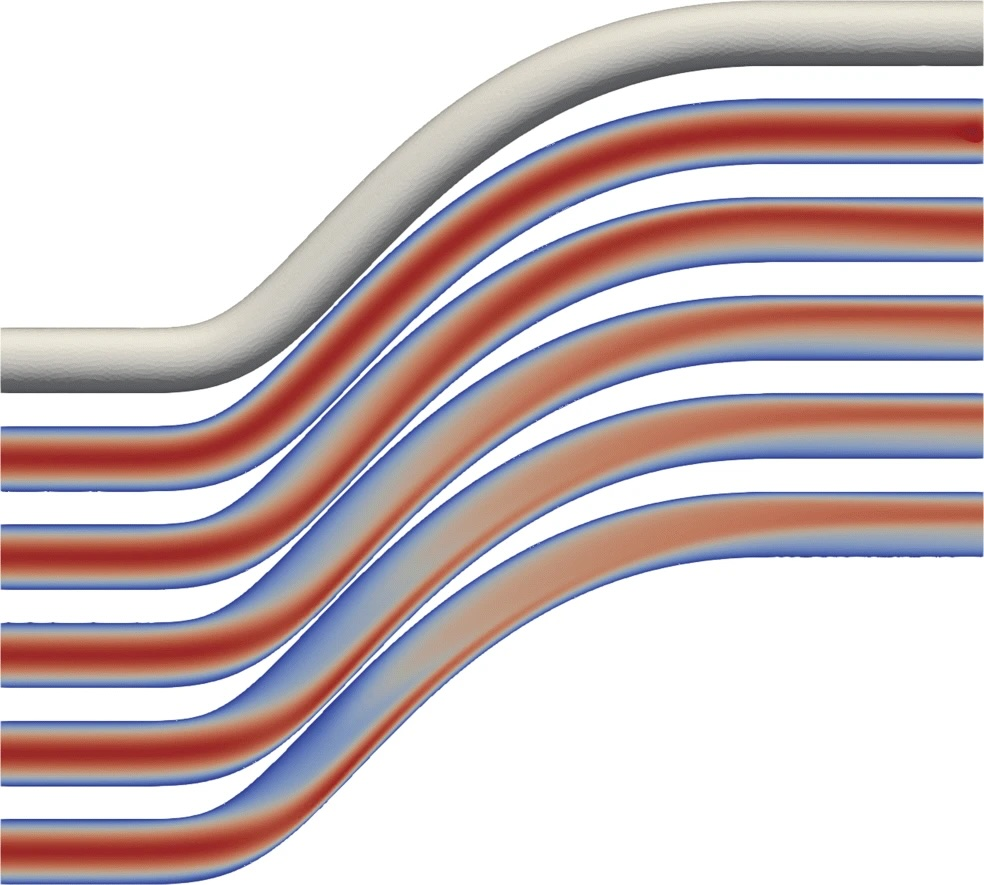
\includegraphics[height=3cm]{pipes}}
}

\end{document}
